\documentclass[]{bioinfo}
\usepackage[table,xcdraw]{xcolor}
\usepackage{caption,subcaption}
\usepackage{hyperref}
\copyrightyear{2014}
\pubyear{2014}

\begin{document}
\firstpage{1}

\title[3Dmol.js: Molecular Visualization with WebGL]{3Dmol.js: Molecular Visualization with WebGL}
\author[Rego and Koes]{Nicholas Rego\,$^{1,2}$ David Koes$^{1}$\footnote{to whom correspondence should be addressed}}
\address{$^{1}$Department of Computational and Systems Biology, University of Pittsburgh, Pittsburgh, PA 15260\\
$^{2}$Department of XXXXXXXX, Address XXXX etc.}

\history{Received on XXXXX; revised on XXXXX; accepted on XXXXX}

\editor{Associate Editor: XXXXXXX}

\maketitle
\begin{abstract}
\section{Summary} 3Dmol.js is a modern, object-oriented JavaScript library that uses the latest web technologies
to provide interactive, hardware-accelerated three dimensional representations of molecular data without the
need to install browser plugins or Java.  3Dmol.js provides a full featured API for developers as well
as a straightforward declarative interface that lets users easily share and embed molecular data in websites.
\section{Availability} 3Dmol.js is distrubuted under the permissive MIT open source license.
Source code and documentation can be found at \url{http://3Dmol.csb.pitt.edu}
\section{Contact:} \href{dkoes@pitt.edu}{dkoes@pitt.edu}
\end{abstract}

\section{Introduction}
Molecular visualization is an essential tool for computational chemists and biologists. Due to the demanding nature of 3D graphics, most molecular viewers, such as PyMol\cite{delano2002pymol}, Chimera\cite{pettersen2004ucsf}, VMD\cite{humphrey1996vmd}, and Avogadro\cite{hanwell2012avogadro}, are desktop applications.  The need to install specialized applications and, in some cases, the restrictive nature of the software licenses, introduces hurdles to the sharing of molecular data.  Unlike a desktop application, a standards-based client-side web application comes pre-installed with every computer and mobile device with a modern web browser and can be seamlessly integrated into online environments for accessing and analyzing molecular data.


Currently, Jmol\cite{jmol,hanson2010jmol} is the most used web-based molecular viewer. Jmol is implemented as a Java applet and includes a custom rendering engine for efficiently rendering common molecular data representations such as spheres and sticks.  Due to this custom rendering engine and Java's optimizing just-in-time compiler, the performance of Jmol can approach that of native, desktop applications.  However, due to heavily publicized security failures, it can no longer be assumed that users have Java installed by default\cite{doomedjava}.  Even when Java is installed, users are presented with multiple security prompts that must be correctly dealt with before a Java applet, such as Jmol, can run.
To address these concerns, JSmol\cite{hanson2013jsmol} was developed. JSmol is largely the result of applying a Java to JavaScript translator to Jmol. As the \textit{de facto} web browser scripting language, JavaScript, unlike Java, is widely deployed and enabled by default.  However, particularly for large and complex visualizations, the performance of JSmol lags behind that of Jmol.

An alternative to the software-based rendering of Jmol/JSmol is to use hardware-accelerated graphics, as is done with desktop applications.  This is enabled by the recently adopted WebGL\cite{webgl} standard, which is now supported by default in the latest versions of all the major desktop and mobile browsers. GLmol\cite{glmol} is a WebGL based molecular viewer that uses the Three.js\cite{threejs} framework for interfacing with WebGL.  However, GLmol lacks a full featured API and the use of the Three.js library results in performance inefficiencies.



\section{3Dmol.js}

3Dmol.js is a pure JavaScript, hardware-accelerated, object-oriented molecular visualization library that enables web developers and casual users to visualize and interact with molecular data in any modern web browser with near native performance.  The goal of 3Dmol.js is not to supplant Jmol/JSmol/GLmol, but to expand the options a

To this end, we have developed 3Dmol.js, based on GLmol, as purely JavaScript (with WebGL), object-oriented molecular visualization library to enable web developers and casual users alike to visualize molecules in a web browser with desktop application like performance.  

Unlike GLmol, 3Dmol.js is a JavaScript library and provides an object-oriented API for developers.  However, 3Dmol.js is also developed with non developers in mind, and contains built in capabilities to meet most users' visualization needs.

By taking advantage of WebGL, 3Dmol.js sidesteps JavaScript's inherent speed limitations and allows fast and smooth image manipulation.  By leveraging native graphics hardware, common image manipulations, including rotating, translating, and zooming are smooth and comparable to Jmol's Java implementation.

3Dmol.js requires installation and can be used immediately by simply including the JavaScript source code.

3Dmol.js provides three main usage scenaries:

\begin{itemize}
\item \emph{For developers}
After including the 3Dmol.js source code, web developers can create applications with 3Dmol's API.

Webmol is also easily embeddable in existing HTML pages.

\item \emph{For collaboration}
3Dmol also provides a collaborative interface, so that users not interested in development can view and share molecules immediately.

\end{itemize}


\begin{figure}
\centering
\begin{minipage}[b]{.9\linewidth}
\begin{subfigure}[b]{\linewidth} \centering
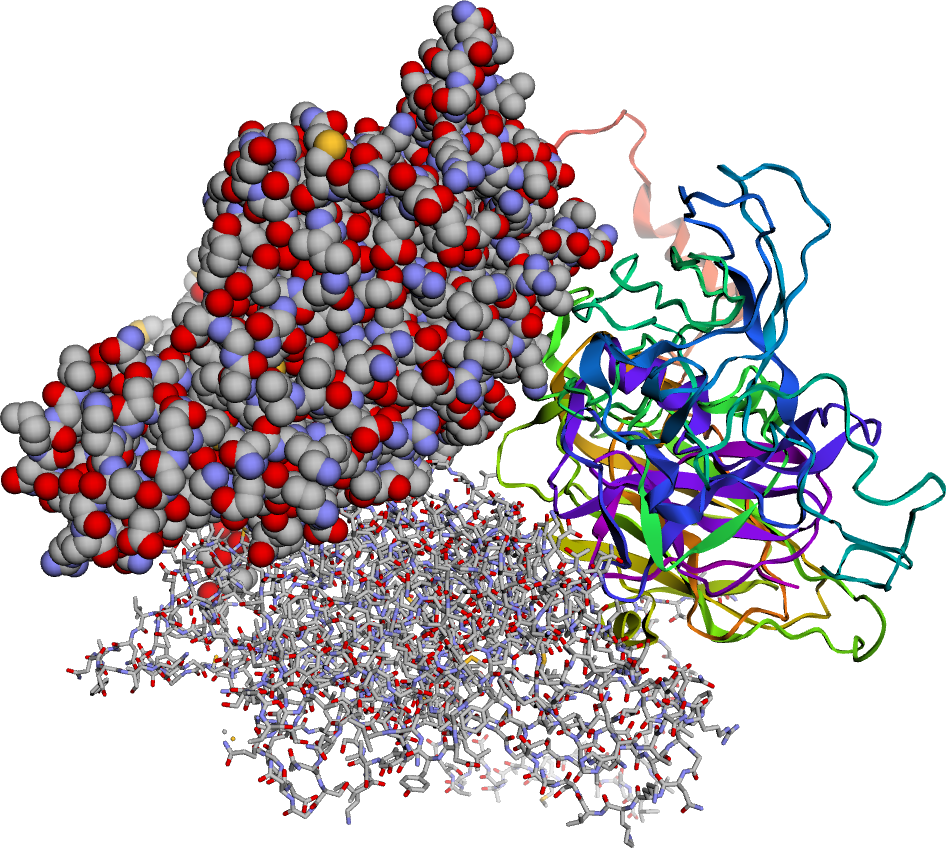
\includegraphics[width=\linewidth]{screenshot}
\caption{}\label{pic}
\end{subfigure}
\end{minipage}

\begin{minipage}[b]{\linewidth}
\begin{subfigure}[b]{\linewidth} \centering
\begin{tabular}{ccccc}
 & \textbf{Jmol} & \textbf{JSmol} & \textbf{GLmol} &\textbf{3Dmol} \\
\textbf{Construct} & \textbf{0.136s} & 0.874s & 6.372s & 0.776s \\
\textbf{Rotate} & 0.053s & 0.207s & 0.673s & \textbf{0.002s} 
\end{tabular}
\caption{}\label{perf}
\end{subfigure}

\begin{subfigure}[b]{\linewidth} \centering
\begin{verbatim}
$3Dmol.download('pdb:3M8L', viewer);
viewer.setStyle({chain:'A'}, {sphere:{} });
viewer.setStyle({chain:'B'}, 
            {cartoon:{color: 'spectrum'} });
viewer.setStyle({chain:'C'}, {stick:{} });
viewer.render();
\end{verbatim}
\caption{}\label{code}
\end{subfigure}

\begin{subfigure}[b]{\linewidth} \centering
\begin{verbatim}
<div style="height: 600px; width: 600px;" 
 class='viewer_3Dmoljs' data-pdb='3M8L'
 data-backgroundcolor='0xffffff'  
 data-select1='chain:A'
 data-style1='sphere'
 data-select2='chain:B'
 data-style2='cartoon:color=spectrum'
 data-select3='chain:C'
 data-style3='stick'></div>
\end{verbatim}
\caption{}\label{embed}
\end{subfigure}

\begin{subfigure}[b]{\linewidth} \centering
\begin{verbatim}
http://3dmol.csb.pitt.edu/viewer.html?
 pdb=3M8L&select=chain:A&style=sphere&
 select=chain:B&style=cartoon:color~spectrum&
 select=chain:C&style=stick
\end{verbatim}
\caption{}\label{url}
\end{subfigure}
\end{minipage}

\end{figure}

\subsection{3Dmol.js JavaScript API}
3Dmol.js provides a high-level JavaScript interface for web developers to create their own visualization applications. 

After including the 3Dmol.js source, all functionality is accessable through the global 3Dmol namespace. 3Dmol uses a GLViewer object instances for individual viewers.  A single webpage can contain multiple viewers.  Each viewer object, in turn, contains any number of model and shape objects.  3Dmol GLModel objects represent molecules, while GLShape objects can represent user-defined generic shapes.

A viewer can be instantiated and attached to an HTML element by calling:


Multiple viewers can be added to separate elements in an HTML file.  A viewer represents molecular structures as collections of atoms in a \emph{GLModel} object.  Multiple models can be added to a single viewer, though a single structure must be contained in one model object.  Models are most easily added to a viewer by reading in a structure file string (currently \emph{PDB}, \emph{sdf}, \emph{mol2}, \emph{xyz}, and Gaussian \emph{cube} formats are supported).  3Dmol can also load PDB structures directly from the RCSB Protein Data Bank.

For instance:

To download a structure with PDB id `2POR' onto viewer from PDB database:



Models can select and apply styles to its atoms, or a viewer can apply styles to atoms matching a certain specification in any of its models.

A viewer instance can select atoms and apply styles on an individual atom basis.  Each viewer has a \emph{render} method to display changes:



\subsection{Embeddable viewer}
Users can also directly embed viewers into HTML elements. This allows users to easily add 3Dmol content to their page by including a single line in their HTML, for instance:


\subsection{Direct molecule viewing with collaborative interface}
3Dmol also provides a URL based viewer that allows users to specify and view a molecule by simply entering a URL into a web browser.  This allows collaborators to share molecular structures by simply navigating to a url in the browser. 

For instance, to immediately view a cartoon representation of a bacterial \emph{porin} protein (PDB ID: 2POR), simply enter the following URL into your browser:

\emph{3Dmol.csb.pitt.edu/viewer.html?pdb=2por\&select=chain\~{}A\&style=cartoon,color\~{}gradient}

\section{Performance Comparisons}



\section*{Acknowledgements}

\paragraph{Funding\textcolon} 
This work was supported by the National Institute of Health [R01GM108340].
The content is solely the responsibility of the authors and does not necessarily
represent the official views of the National Institute of General Medical Sciences
or the National Institutes of Health.

\bibliographystyle{plain}
\bibliography{3dmol}
\end{document}